\chapter{Rastreabilidade}

\label{sec:rastreabilidade}
Previamente definida a estratégia de rastreabilidade no planejamento a ser seguido dentro projeto original, foi levantada a utilização de uma matriz de rastreabilidade, para fornecer e auxiliar na visibilidade do projeto, sendo que por meio desta matriz sería possível obter a origem dos itens de rastreabilidade, também previamente definidos no planejamento inicial do projeto, partindo do problema, necessidade, característica e requisitos, que estão documentados, sendo eles os elos de rastreabilidade que definiram o relacionamento dentro das matrizes de rastreabilidade descritas nas secções deste capítulo. Os itens de rastreabilidade  das tabelas deste capitulo estão definidos por \textit{Tags}.


\section{Necessidades x Características}

Como está referenciado na tabela \ref{nc-ch}, as caracteristicas da coluna a extrema esquerda correspondem a quais necessidades do cliente especificadas na linha superior. Neste caso especifico para o este projeto, a relação entre estes itens de rastreabilidade é de que uma necessidade possui várias caracterísitcas e uma caracteristica está vinculada a uma necessidade.

\begin{table}[H]
  \centering
  \caption{Matriz de rastreabilidade: necessidades x características}
  \label{nc-ch}
  \begin{tabular}{|l|l|l|l|l|}
    \hline
         & NC1 & NC2 & NC3 & NC4 \\ \hline
    CH1  &  X   &     &     &     \\ \hline
    CH2  &  X   &     &     &     \\ \hline
    CH3  &  X   &     &     &     \\ \hline
    CH4  &  X   &     &     &     \\ \hline
    CH5  &     &  X   &     &     \\ \hline
    CH6  &     &  X   &     &     \\ \hline
    CH7  &     &     &  X   &     \\ \hline
    CH8  &     &     &  X  &     \\ \hline
    CH9  &     &     &  X   &     \\ \hline
    CH10 &     &     &  X   &     \\ \hline
    CH11 &     &     &  X   &     \\ \hline
    CH12 &     &     &  X   &     \\ \hline
    CH13 &     &     &  X   &     \\ \hline
    CH14 &     &     &     &   X  \\ \hline
    CH15 &     &     &     &   X  \\ \hline
    CH16 &     &     &     &   X  \\ \hline
    CH17 &     &     &     &   X  \\ \hline
    CH18 &     &     &     &   X  \\ \hline
    CH19 &     &     &     &   X  \\ \hline
    CH20 &     &     &     &   X  \\ \hline
    CH21 &     &     &     &   X  \\ \hline
    CH22 &     &     &     &   X  \\ \hline
    CH23 &     &     &     &   X  \\ \hline
  \end{tabular}
\end{table}

\section{Características x Requisítos Funcionais}

Como está referenciado na tabela \ref{ch-rf}, os requisitos da coluna a extrema esquerda estão relacionados a quais caracteristicas especificadas na linha superior. Caracteristicas nas quais são relacionadas as necessidades do cliente, o que torna uma rastreabilidade indireta entre os requisitos e as necessidades do cliente. Neste caso especifico para este projeto, a relação entre estes itens de rastreabilidade é de que uma característica possui vários requisitos e um requisito está vinculada a uma característica.

\begin{table}[H]
\tiny
\centering
\caption{Matriz de rastreabilidade: características x requisítos funcionais}
\label{ch-rf}
\begin{tabular}{|l|l|l|l|l|l|l|l|l|l|l|l|l|l|l|l|l|l|l|l|l|l|l|l|}
\hline
&\begin{turn}{90}CH01 \ \end{turn} & \begin{turn}{90}CH02 \ \end{turn} & \begin{turn}{90}CH03 \ \end{turn} & \begin{turn}{90}CH04 \ \end{turn} & \begin{turn}{90}CH05 \ \end{turn} & \begin{turn}{90}CH06 \ \end{turn} & \begin{turn}{90}CH07 \ \end{turn} & \begin{turn}{90}CH08 \ \end{turn} & \begin{turn}{90}CH09 \ \end{turn} & \begin{turn}{90}CH10 \ \end{turn} & \begin{turn}{90}CH11 \ \end{turn} & \begin{turn}{90}CH12 \ \end{turn} & \begin{turn}{90}CH13 \ \end{turn} & \begin{turn}{90}CH14 \ \end{turn} & \begin{turn}{90}CH15 \ \end{turn} & \begin{turn}{90}CH16 \ \end{turn} & \begin{turn}{90}CH17 \ \end{turn} & \begin{turn}{90}CH18 \ \end{turn} & \begin{turn}{90}CH19 \ \end{turn} & \begin{turn}{90}CH20 \ \end{turn} & \begin{turn}{90}CH21 \ \end{turn} & \begin{turn}{90}CH22 \ \end{turn} & \begin{turn}{90}CH23 \ \end{turn} \\ \hline
RF01&   X   &      &      &      &      &      &      &      &      &      &      &      &      &      &      &      &      &      &      &      &      &      &      \\ \hline
RF02&   X  &      &      &      &      &      &      &      &      &      &      &      &      &      &      &      &      &      &      &      &      &      &      \\ \hline
RF03&      &   X   &      &      &      &      &      &      &      &      &      &      &      &      &      &      &      &      &      &      &      &      &      \\ \hline
RF04&      &      &   X   &      &      &      &      &      &      &      &      &      &      &      &      &      &      &      &      &      &      &      &      \\ \hline
RF05&      &      &      &   X   &      &      &      &      &      &      &      &      &      &      &      &      &      &      &      &      &      &      &      \\ \hline
RF06&      &      &      &   X   &      &      &      &      &      &      &      &      &      &      &      &      &      &      &      &      &      &      &      \\ \hline
RF07&      &      &      &      &   X   &      &      &      &      &      &      &      &      &      &      &      &      &      &      &      &      &      &      \\ \hline
RF08&      &      &      &      &      &    X  &      &      &      &      &      &      &      &      &      &      &      &      &      &      &      &      &      \\ \hline
RF09&      &      &      &      &      &    X  &      &      &      &      &      &      &      &      &      &      &      &      &      &      &      &      &      \\ \hline
RF10&      &      &      &      &      &    X  &      &      &      &      &      &      &      &      &      &      &      &      &      &      &      &      &      \\ \hline
RF11&      &      &      &      &      &      &   X   &      &      &      &      &      &      &      &      &      &      &      &      &      &      &      &      \\ \hline
RF12&      &      &      &      &      &      &      &   X   &      &      &      &      &      &      &      &      &      &      &      &      &      &      &      \\ \hline
RF13&      &      &      &      &      &      &      &   X   &      &      &      &      &      &      &      &      &      &      &      &      &      &      &      \\ \hline
RF14&      &      &      &      &      &      &      &   X   &      &      &      &      &      &      &      &      &      &      &      &      &      &      &      \\ \hline
RF15&      &      &      &      &      &      &      &   X   &      &      &      &      &      &      &      &      &      &      &      &      &      &      &      \\ \hline
RF16&      &      &      &      &      &      &      &      &   X   &      &      &      &      &      &      &      &      &      &      &      &      &      &      \\ \hline
RF17&      &      &      &      &      &      &      &      &      &   X   &      &      &      &      &      &      &      &      &      &      &      &      &      \\ \hline
RF18&      &      &      &      &      &      &      &      &      &   X   &      &      &      &      &      &      &      &      &      &      &      &      &      \\ \hline
RF19&      &      &      &      &      &      &      &      &      &      &    X  &      &      &      &      &      &      &      &      &      &      &      &      \\ \hline
RF20&      &      &      &      &      &      &      &      &      &      &      &   X   &      &      &      &      &      &      &      &      &      &      &      \\ \hline
RF21&      &      &      &      &      &      &      &      &      &      &      &      &   X   &      &      &      &      &      &      &      &      &      &      \\ \hline
RF22&      &      &      &      &      &      &      &      &      &      &      &      &      &   X   &      &      &      &      &      &      &      &      &      \\ \hline
RF23&      &      &      &      &      &      &      &      &      &      &      &      &      &      &   X   &      &      &      &      &      &      &      &      \\ \hline
RF24&      &      &      &      &      &      &      &      &      &      &      &      &      &      &      &   X   &      &      &      &      &      &      &      \\ \hline
RF25&      &      &      &      &      &      &      &      &      &      &      &      &      &      &      &      &   X   &      &      &      &      &      &      \\ \hline
RF26&      &      &      &      &      &      &      &      &      &      &      &      &      &      &      &      &   X   &      &      &      &      &      &      \\ \hline
RF27&      &      &      &      &      &      &      &      &      &      &      &      &      &      &      &      &      &   X   &      &      &      &      &      \\ \hline
RF28&      &      &      &      &      &      &      &      &      &      &      &      &      &      &      &      &      &      &   X   &      &      &      &      \\ \hline
RF29&      &      &      &      &      &      &      &      &      &      &      &      &      &      &      &      &      &      &      &   X   &      &      &      \\ \hline
RF30&      &      &      &      &      &      &      &      &      &      &      &      &      &      &      &      &      &      &      &      &   X   &      &      \\ \hline
RF31&      &      &      &      &      &      &      &      &      &      &      &      &      &      &      &      &      &      &      &      &      &  X    &      \\ \hline
RF32&      &      &      &      &      &      &      &      &      &      &      &      &      &      &      &      &      &      &      &      &      &   X   &      \\ \hline
RF33&      &      &      &      &      &      &      &      &      &      &      &      &      &      &      &      &      &      &      &      &      &      &  X    \\ \hline
RF34&      &      &      &      &      &      &      &      &      &      &      &      &      &      &      &      &      &      &      &      &      &      &  X    \\ \hline
RF35&      &      &      &      &      &      &      &      &      &      &      &      &      &      &      &      &      &      &      &      &      &      &  X    \\ \hline
\end{tabular}
\end{table}

\section{Rastreabilidade na ferramenta : \textit{Innoslate} }

Como foi proposto no planejamento inicial, foi utilizada uma ferramenta para manter documentado todos os itens de rastreabilidade que seriam trabalhados durante o projeto original. Denominada Innoslate, essa ferramenta possui o suporte necessário para armazenamento dos itens de rastreabilidades previamente selecionados, porém não fornece suporte para a aplicação da matriz de rastreabilidade, o que reforçou o fato de documenta-la neste capítulo. Por se tratar de uma ferramenta com acesso via internet e possuir suporte para trabalho colaborativo, foi mantida a total visibilidade de todos os itens por todo os integrantes do grupo, atingindo assim, o objetivo firmado para a utilização desta ferramenta.

\begin{figure}[H]
  \center
  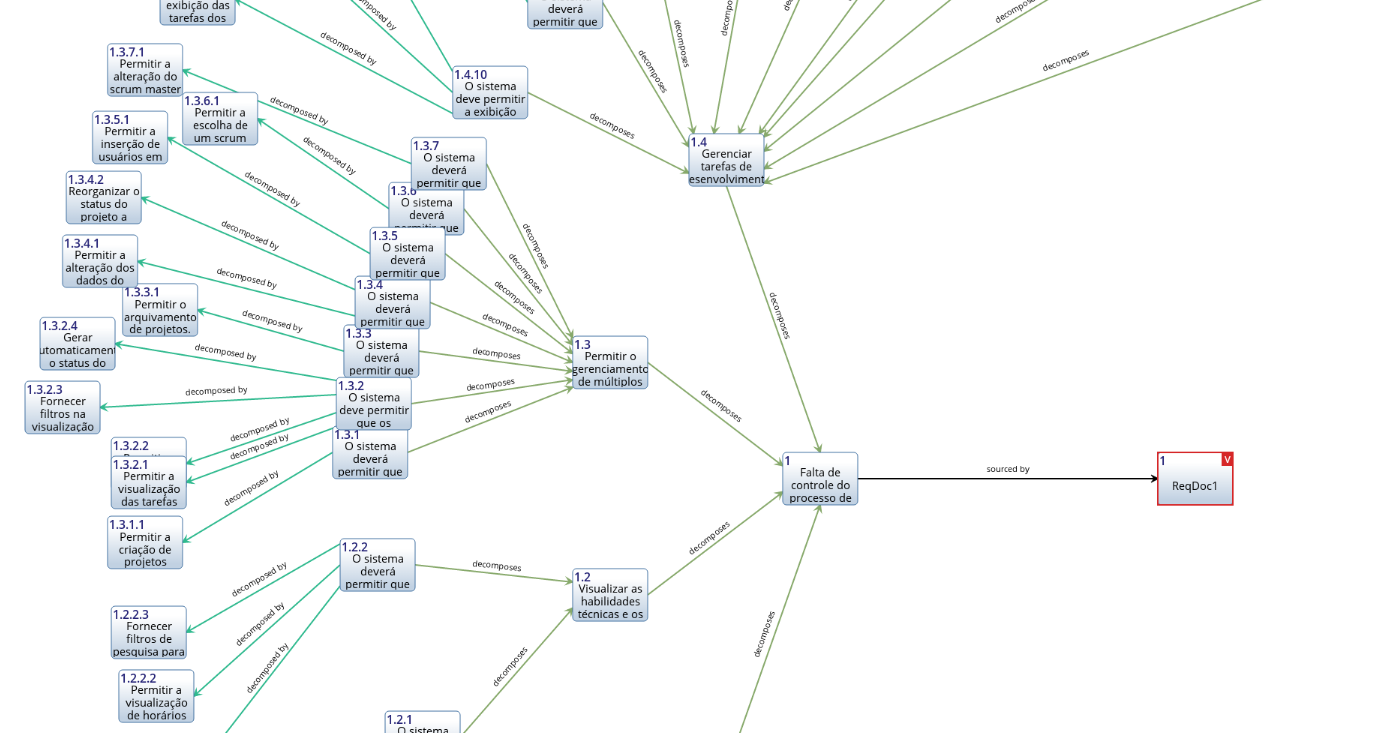
\includegraphics[width=0.8\textwidth]{figuras/spider.png}
  \caption{Diagrama de spider para rastreamento}
  \label{fig:diagrama-caso-uso}
\end{figure}

\begin{figure}[H]
  \center
  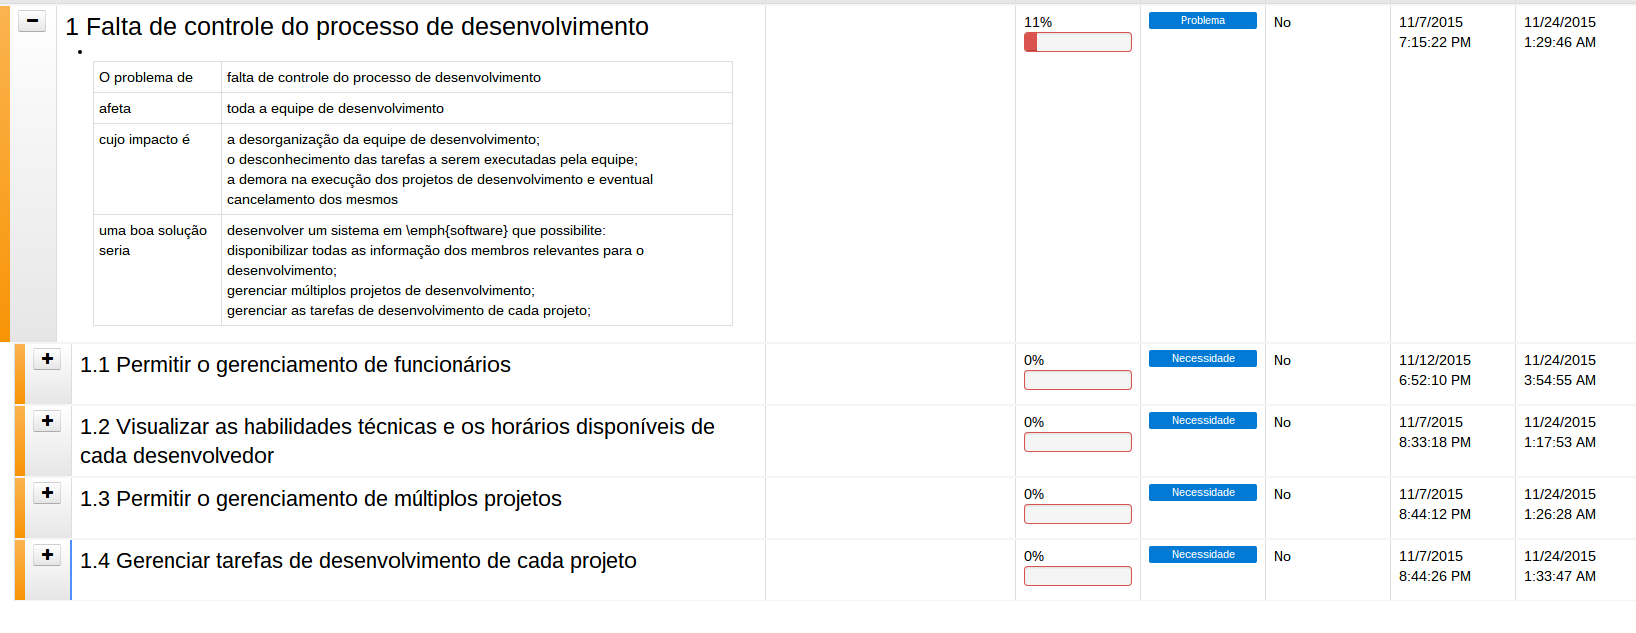
\includegraphics[width=0.8\textwidth]{figuras/necessidades.png}
  \caption{Ferramenta mostrando Problema e Necessidades}
  \label{fig:diagrama-caso-uso}
\end{figure}

\begin{figure}[H]
  \center
  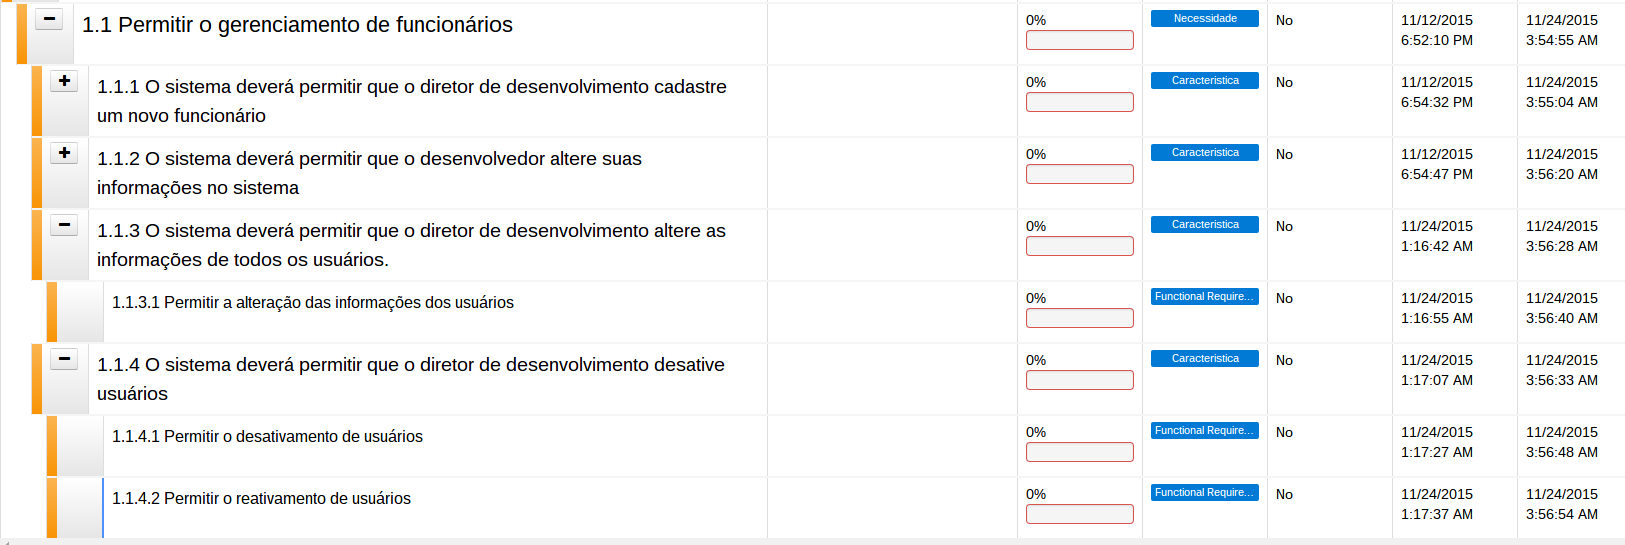
\includegraphics[width=0.8\textwidth]{figuras/carac-req-fun.png}
  \caption{Ferramenta mostrando Necessicade, caracteristicas e requisitos funcionais}
  \label{fig:diagrama-caso-uso}
\end{figure}

